%! Author = NekoHitDev
%! Date = 2021/7/30
%! Language = English (US)
%! compiler = XeLaTex

% Preamble
\documentclass[12pt,a4paper]{article}
\usepackage[T1]{fontenc}

% Packages
\usepackage{amsmath}
\usepackage{url}
\usepackage{graphicx}
\usepackage[slantfont, boldfont]{xeCJK}

% set CJK font
\setCJKmainfont[FallBack=SimSun-ExtB]{SimSun}

% include header file
\newcommand{\editversion}{v0.0.1-RC1}

\newcommand{\gentitlepage}[1]{
    \begin{titlepage}
        \centering
        \vfill
        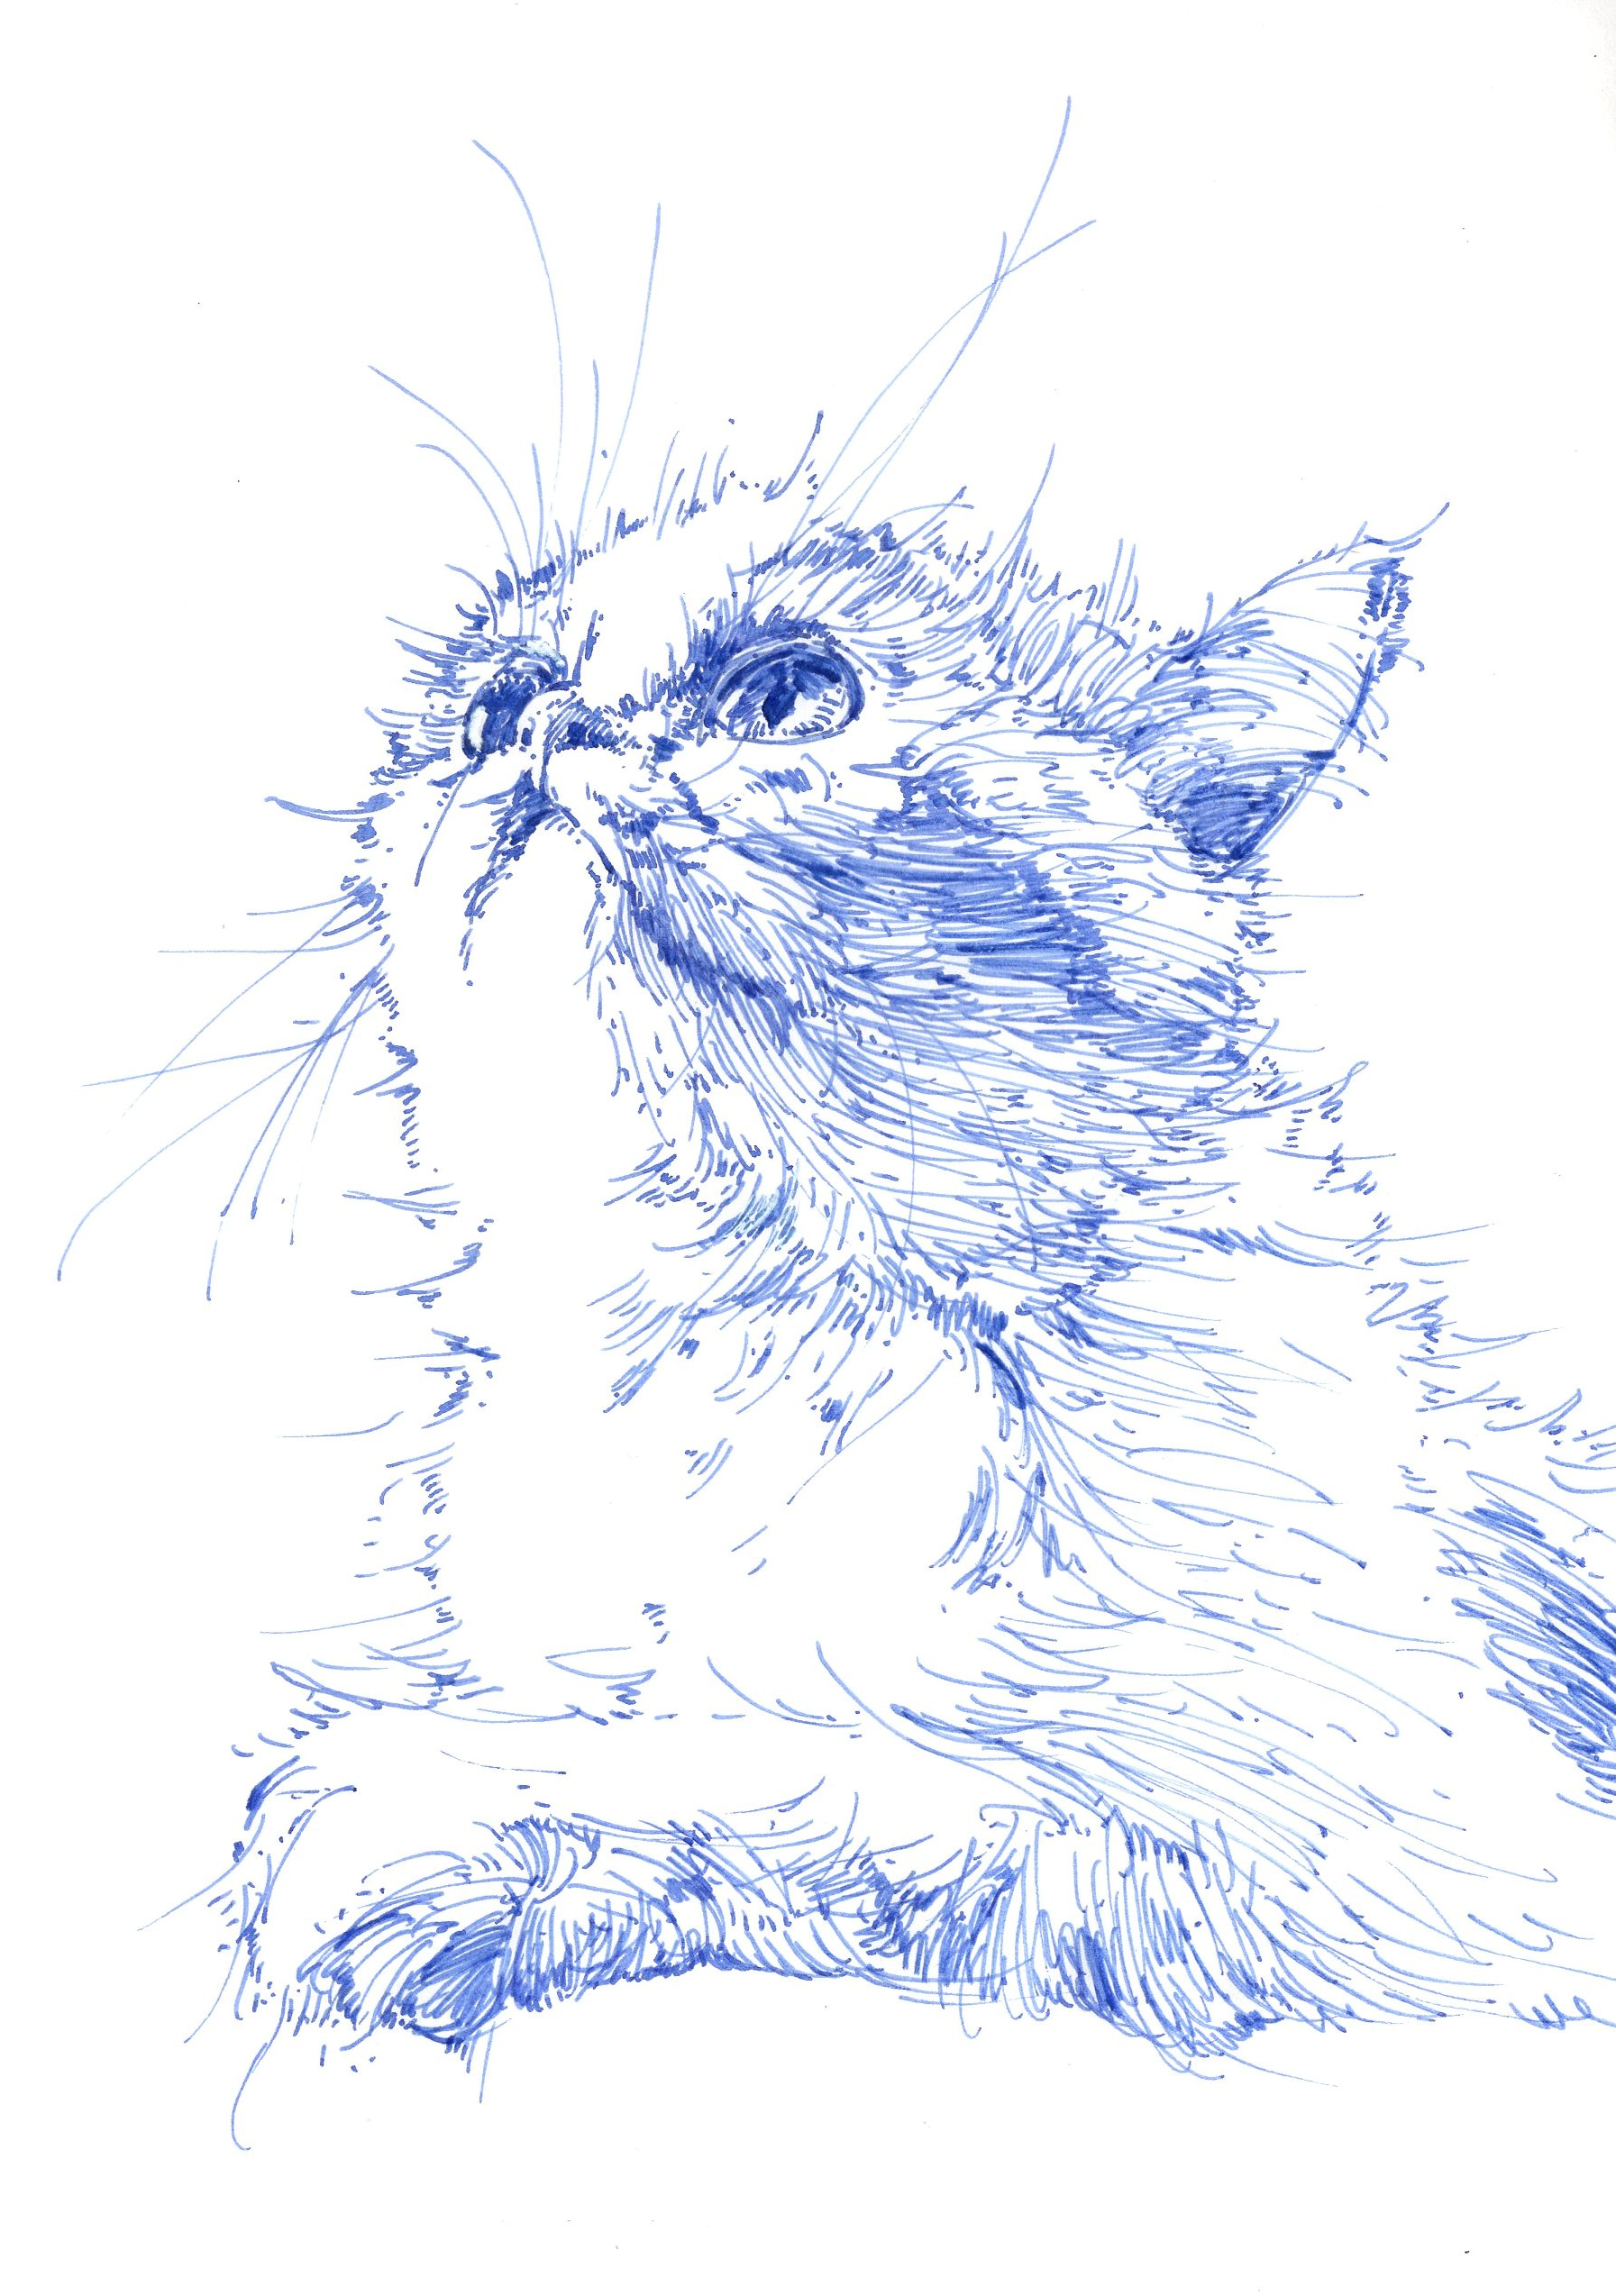
\includegraphics[width=0.8\textwidth]{assets/img196}
        \vfill
        {\Huge
        \textsf{NekoHit Project}\\
        #1\\
        \vskip2cm
        \vfill
        \Large
        \editversion
        }
        \vfill
        \vfill
    \end{titlepage}
}

% TOC stop at subsection
\setcounter{tocdepth}{2}


% Document
\begin{document}
    \gentitlepage{White paper}

    \pagenumbering{Roman}
    \tableofcontents
    \vspace*{\fill}
    \begin{center}
        
\includegraphics[width=0.67\textwidth]{assets/img197}
    \end{center}
    \clearpage

    \pagenumbering{arabic}


    \section{Vision of the future}\label{sec:goal}
    The vision (goal) of the NekoHit Project is to build a decentralized
application that gives creators the freedom to spend their time and energy,
and allows audiences to support creators financially while incentivizing
creators to respond to sponsors.

As more and more creators and sponsors join, we envisioned that the NekoHit
community would grow and improve.
We, the developers of this project, will respond to the needs and feedback
from the community and do our best to create an energetic platform for creators.


    \section{Introduction}\label{sec:intro}
    The NekoHit Project was built on top of the work completion agreement (WCA
for short).
The project aims to incorporate \textit{insurance} into the traditional sponsor
model, promote audiences' willingness to support content creators financially,
and motivate creators to comply with their promises and finish the project
on time.

NekoHit Project use a project-based sponsor model.
Instead of paying a monthly subscription fee, we allow the audience to sponsor
a project more precisely.
To gain the audience's trust, content creators need to pledge (stake) some
tokens first.
These tokens need to be transferred to our WCA smart contracts before the
sponsors can transfer the tokens to the creator's projects for sponsorship.
Our WCA contract also holds the sponsored tokens.
When declaring a project, the creator needs to provide information such as
the staking (pledging) rate, detailed milestones, and the expected completion
time.
Suppose the creator does not complete certain milestones by the scheduled time.
In that case, the WCA contract will automatically calculate the percentage of
those milestones to the project and deduct it from the pre-pledged tokens.
After the project is completed, the deducted tokens will be released to each
sponsor in proportion to the reference sponsorship amount.
Also, tokens sponsored by sponsors will be deducted by the corresponding
percentage and returned to the sponsor's wallet as a refund.
So not only does the author not receive the sponsorship tokens for his defaulted
milestone, but he also loses some of his own pledged tokens.

We use this mechanism as a safety net to protect our sponsors' rights and
incentivize creators to complete their projects in time.
Such a mechanism will also urge the creators to think carefully about the
project and arrange the timeline appropriately.
Last but not least, we hope that this will increase the audience's trust in
the content creators and reduce their concerns about financial sponsorship.



    \section{Industry Status}\label{sec:now}
    There is a growing interest in the creator economy, where audiences are
willing to fund creators, and creators also need various sources of income
to sustain their work.

Currently, two famous models are widely used on the market: subscription-based
model and crowdfunding-based model.

The typical platform using the subscription-based model is Patreon.
It is based on a monthly subscription model, where creators can customize
their plans at different prices.
Usually, the lower price means fewer returns, and higher the price, more 
returns you get.
Subscription-based model requires creator has already finish part of his work,
meanwhile having reasonable updates to response their supporters.
Once supporters not satisfied with the update, they can only stop the subscription,
and can't do much about the already paid subscription.

Kickstarter is a platform using the crowdfunding-based model.
It prefers a one-time sponsorship compared to Patreon's monthly subscription.
Just like Patreon, creator can set up different returns for different amount.
According to Kickstarter's introduction\cite{kickstarter_about}, the platform
is dedicated to transforming creative ideas into reality.
The initiator (creator) of a crowdfunding project will have complete control
over the works.
Kickstarter favors creators by giving them as much freedom as
possible to turn excellent creative ideas into real-world products.
Such independence can inspire superior products, but supporters can do
nothing when they realize they have been fooled in malicious projects.

The traditional crowdfunding model puts all the initiative on the creator.
Once the sponsor pays the sponsored money, they have no control over the
project, no matter it can be completed, or be refunded, or never updated again.
For a monthly subscription model, sponsors can stop subscribing from
next month.
However, for sponsors already subscribed, the only thing they can do is stop
the subscription if the creator doesn't do anything or delivered less-quality
works.

As a conclusion, in current sponsor models, supporters are in a weak position
where they cannot protect their right in an efficient way when dealing with
malicious creator.
This type of creator can be hard to locate and uncover, thus the existence of them
make supporters trust less when facing a freshmen and preventing fresh creators
to start their project.



    \section{Our solution}\label{sec:solution}
    In the previous section, we concluded the disadvantages of two models on the market.
We intend to solve those trust issues with the NekoHit Project.
The project consists of three key components: the work completion agreement
(WCA), the completion agreement tokens (CAT), and the Nekoin token for community DAO\@.
Our project focused on implementing a sponsorship platform that is simple and
easy to use.
Meanwhile, gives users (both creators and sponsors) the power and ability to
protect their rights and interests.
During the process, we want to be as open as possible: we do not restrict
what platform the creator uses to store the work, nor specify how users invoke
our contracts. Now with the help from Flamingo, we have no limitations on what
token our users want to use when pledging and sponsoring.

\subsection{Work Complete Agreement}\label{subsec:wca}

The Work Completion Agreement (WCA) is the core feature of the NekoHit Project.
WCA is based on individual projects and gives sponsors more control compared
to existing models.
In addition to be able to making a refund \footnote{
    Refunds depend on the progress of the project and
    in some cases full refunds are not possible.
} at any time, it also provides an insurance-like mechanism that automatically
refunds to the sponsor's wallet after the creator failed to meet the schedule
and penalizes the creator.
The WCA is implemented as a smart contract.

\subsubsection{Concepts explanation}

\paragraph{Project}

Refers to activities initiated by creators in the real world, such as the production
of novels, illustrations, or other works.
The project is recorded as a series of data in the WCA contract, such as the
address of the creator, the milestone definitions.
Each project has a unique textual identifier for the user uniquely specifies a
certain project when interacting with the contract.

\paragraph{Milestone}

Each project contains at least 1 milestone.
The milestone reflect the important event in the project.
For a periodic project, milestones can represent the updates in current period.
For a one-time project, milestones can be key events in the project.
NEP-17 assets will be accounted according to milestones' status.

Each milestone has a expected completion time.
The creator can only mark the milestone as finished before this time, otherwise
it will be considered as violated.
When violating a milestone, a portion of supported token will be refunded to supporters,
and part of the pledged token will be transferred supporters as a compensation.

\paragraph{Threshold milestone}

The creator specifies a milestone as the threshold milestone.
By its meaning, the participants of this project can make a regret before this
milestone is reached (marked as finished or violated).
The creator can cancel this project without losing anything, and every supporter
can get a full refund.
After reach this milestone, the creator cannot cancel this project.
Finish the project anyway will cause him/her/they lose large part of the pledged
token, and cannot get the supported token from supporter.
Also, supporters cannot do full a refund anymore, once the project reached the
threshold milestone, all finished milestones will be paid, only a partial refund
can be achieved.

\paragraph{Cooldown interval}

The creator must invoke the contract to mark a milestone as finished.
During this process, the creator must set up a cooldown time to ensure
at least this amount of time has been passed between two updates.
The goal of this interval is to protect supporters from malicious creator,
who wants to quickly finish all milestones and take away the tokens.
By introducing the cooldown interval, supporters can have enough time to
exam the update and make a refund if they think they are spammed.
However, different project requires different interval, this parameter is defined
by the creator and display it clearly when the sponsor browsing the project.
It is up to the sponsor to decide whether to believe a given cooldown interval.

\paragraph{The maximum amount of sponsorship}

Unlike existing model, WCA defined a maximum amount of sponsorship to ensure
every supporter will get a reasonable compensation when creator violate milestones.
The sponsored tokens from all sponsors on this project cannot exceed that value.

\paragraph{Stake (pledge) rate}

Will determine the pledge's total amount and the payout ratio when the
creator misses a milestone.

\paragraph{Status and stages}

WCA use status to statically mark a project for a easier way to manage the
lifecycle of the it.
For example, when you request a refund, the project status must not be `finished`
or `pending`.
Status is only changed when user interact with the project.
For example, the status will be changed from `pending` to `ongoing` when creator
pledged the correct amount of token.

Every status has 0 or more stages.
Stages are dynamically computed.
For example, `ongoing` status has stages like: `OPEN` (where the threshold
milestone is not reached), `ACTIVE` (where the threshold milestone is reached)
and `ReadyToFinish` (where the last milestone is reached, but tokens are still
held by the contract).
Different operations will require different status and stage, some operations will
have different action on different status and stage.

\subsubsection{Overview}

One complete use process of the WCA is as follows:

\begin{enumerate}
    \item The creator calls the WCA contract to declare a project
    \item The creator calls the NEP-17 contract to transfer pledged tokens
    \item Supporters call the same NEP-17 contract to transfer sponsored tokens
    to the project\label{item:purchase_wca}
    \item The creator calls the WCA contract to update the project (update
    milestone)\label{item:update_milestone}
    \item The creator or sponsor calls the WCA contract to end the project
    (accounting tokens)\label{item:finish_project}
\end{enumerate}

Step~\ref{item:update_milestone} can be called multiple times by the creator
to update different milestones.
The sponsor can make a refund anytime, from the moment he starts his sponsorship
at step~\ref{item:purchase_wca} until the end of the project before
step~\ref{item:finish_project}.
However, the refund amount can vary from complete to partial, depending on
the project's progress.

\subsubsection{Declare project}

Declaring a project refers to bind the given project information with the
unique identifier and register it to the WCA contract.
Currently, you cannot change the info after registered the project.
In the future we will implement a voting mechanism to let the supporters approve
or disapprove creator's requests to change milestone settings.

\subsubsection{Stake (pledge) token}

Staking token is required after the creator declares his project by transferring
the specified amount of tokens to the WCA contract before allowing the sponsor
to purchase it.
If anyone attempts to sponsor or operate an unpaid project, the contract will
throw an exception and make the transaction invalid.

The calculation formula of the specified amount is as follows:
$\text{total stake} = \text{stake rate} \times \text{maximum amount of sponsorship}$

Assuming A project with the maximum sponsorship amount of 1000 tokens and
the stake rate is 0.5. A total of 500 tokens will be required.

Currently, the WCA contract supports all NEP-17 tokens, but to keep users away
from fraud, we only list tokens approved by our community (like NEO, GAS, CAT,
fUSDT, FLM, etc.).

\subsubsection{Sponsor a project}

After creators complete the stake, they can advertise their projects on other
platforms.
Sponsors can sponsor the project using the identifier.

When making the sponsor, you have to transfer tokens to the WCA contract with
the identifier as the fourth parameter (aka the data param), so the contract
can record your sponsorship to this specific project.
If the identifier does not exist or is not available for purchase, the contract
will throw an exception to make this transaction invalid, and your assets will be safe.

A project is available to sponsor only if: the creator has paid the stake
and the last milestone has not been completed nor violated.

\subsubsection{Updating project}

The creator may invoke the WCA contract at any time to update the milestone
of the project.
Only subsequent milestones are allowed to update, and the creator cannot
update the already passed milestones.

For example, Milestone \#1 and \#3 are finished, so milestone \#2 cannot be
updated even if it is not expired.

A piece of text is required when updating the milestone.
Since the storage fee is expensive on the blockchain, we don't recommend keeping
your work directly on the blockchain.
This text can be a URL, or an IPFS CID, or a piece of description that guides
your sponsors to find your work.
If the sponsor fails to find your work through this text, they may assume that
the creator started completing the milestone maliciously and consider a refund.
The creator can not modify milestones once they are updated, so please
double-check this text before formally approve the transaction.

Also: all data stored on the Neo N3 blockchain is open and transparent, which
means that your text can be accessed by anyone (including previously refunded
sponsors).
We are planning to solve this by using NeoFS's ACL\@.

\subsubsection{Refund}

Sponsors can initiate a refund at any time before the end of the project,
and the contract will automatically process the refund without waiting for
the consent of the administrator or creator.
The specific refund rules are as follows:

Suppose the threshold milestone has not been completed.
In that case, you can make a full refund at any time, and your sponsor record
will be deleted after the refund.
The creator will not be aware of your refund unless he reviews the transaction
record of the blockchain.

Suppose the threshold milestone has already been passed (in the meaning of
violated or finished by creator).
In that case, you can only get the proportion corresponding to the milestones
that the creator has not yet completed.
Take the following project as an example: there are ten milestones, the first
one is \#1, the last one is \#10, and the threshold milestone is \#3.
Milestone \#1, \#2 and \#4 are finished, milestone \#3 and the rest of them
have not been completed.
Since milestone \#4 has been achieved, the threshold milestone \#3 will be
considered as reached, so only a partial refund is applicable.

The refund ratio is: 3 out of 10 is completed by the creator.
The WCA Contract will send 30\% of the sponsored token directly to the creator.
The remaining 70\% will be refunded to the sponsor's address.

At the final accounting, milestone \#3 will be considered as unfinished.
Thus, 10\% of the pledged tokens will be distributed in proportion to
each sponsor's amount, but this is not applicable when processing the refund,
aka no punishment for the creator when doing the refund.

\subsubsection{Ending the project}

Ending the project will trigger the WCA contract to account for the property
and transfer tokens to each related account.
Please take the following project as an example: the maximum sponsorship amount
is 5000, the stake rate is 0.2, there are ten milestones in total, and the
creator completed seven of them, the creator staked 1000 tokens.

User A sponsored 500 tokens, user B sponsored 1000 tokens, and user C sponsored
300 tokens.

When doing the accounting, the stake amount corresponding to user A is
$500 \times 0.2 = 100$ tokens, so the total amount of user A is 500 tokens
sponsored and 100 tokens staked from the creator, a total of 600 tokens.
The creator didn't finish three milestones, so 30\%, aka 180 tokens, will be
transferred to user A\@.
Similarly, user B will receive a refund of 360 tokens, and user C will receive
108 tokens.

For the part that returned to the creator, it is calculated as follows: the
staked part plus the total sponsored amount, i.e.,
$1000 + 500 + 1000 + 300 = 2800$ tokens, subtract those tokens transferred
to the sponsor, the remaining $2800 - 180 - 360 - 108 = 2152$ tokens, which
will be transferred to the creator in one transaction to save GAS\@.

Updating the last milestone will automatically trigger this process.

\subsubsection{Canceling the project}

Canceling a project is deleting project logically. After the cancellation,
the WCA contract will completely forget everything about that project, but
the transaction where you declare the project will still exist on the blockchain
physically.

Canceling projects allows the creator to make a regret. Canceling project will
remove all related data in the contract storage area, after that, the creator
can create another project with the same identifier. However, this operation
can be only used before the project across the threshold milestone.
For projects haven't staked or pledged yet, cancel a project is basically delete
data. For projects have already staked or pledged, the WCA contract will automatically
handle the refund. At this time, full refund is applied and no punishment is applied.
For the rest of projects, the WCA contract will reject the cancel request.

\subsection{Completion Agreement Token}\label{subsec:cat}

Completion Agreement Token (CAT) is a circulation token issued by NekoHit Project.
Currently, CAT token is a plain NEP-17 token, but in the future, we will implement
features like auto-pay.

The goal of CAT token is to fully eliminate the marketing fluctuations.
CAT token should be used to sponsor content creators in NekoHit Project, thus
we decide to fix the exchange rate and open the ability to issue new tokens to
everyone.
The exchange rate of CAT token is: 1 CAT = 0.5 USD wrapped coin.
The total supply amount is not fixed, and the token has a precision of two
decimal places, in line with the real world legal tender.
User can send some amount of USD wrapped coin to CatToken contract, the contract
will calculate the corresponding amount of CAT token and record to sender's address.
User can also invoke CatToken contract to destroy some amount of CAT token, the
contract will calculate the amount of USD wrapped coin and transfer to caller's
address.

Now the USD wrapper coin is fUSDT, which is Flamingo's USDT wrapper.

\subsection{Community DAO token}\label{subsec:nekoin}

The Nekoin (combination of `neko` and `coin`) is the community DAO token for
the NekoHit Project.
A voting mechanism will be implemented to decide which features are good to have,
and which features can be removed, etc.
Holding the token means you are a member of the community and has the right to
decide where NekoHit Project will go.
The token has no value guaranteed.
You can exchange it with other coins, but this is not part of the design.



    \section{Roadmap}\label{sec:roadmap}
    Currently, we have the following roadmap:

\begin{itemize}
    \item December 2021
    \begin{itemize}
        \item Main net deployment (CatToken and WCA Contract v1.0.0)
        \item Release frontend for main net
        \item Airdrop event and advertising
    \end{itemize}

    \item January 2022
    \begin{itemize}
        \item Airdrop event and advertising
    \end{itemize}

    \item February 2022
    \begin{itemize}
        \item Implement NekoinToken with voting mechanism
    \end{itemize}

    \item March 2022
    \begin{itemize}
        \item Release update v1.1.0 with feedback from the community
        \item Main net deployment (v1.1.0 and NekoinToken)
    \end{itemize}
\end{itemize}



    \section{Epilogue}\label{sec:end}
    \begin{quotation}
    "NekoHit" was just a random name that translates into "cat punch".
    The project was born out of a sudden idea from an unknown novel author
    (Wakayume) while walking.
    After talking with a programmer who had just tried blockchain development
    (Sky Blond) at Misskey.
    The project took a very primitive shape after a simple development.

    Then we went to a hackathon organized by the Neo foundation.
    The original purpose was to have a try.
    And during that contest, we met Yannick Koitzsch, a great teammate doing
    the development along with us.
    In the end, it was a great honor that we received the excellence award
    from the Neo Frontier Launchpad.

    I know that we and NekoHit Project are still very young and inexperienced.
    But because we have tried and worked hard, we have been able to grow and
    evolve during the process.
    I would also like to thank everyone who has supported and encouraged us.
    Because of you, we can keep going.

    The excellence award from Neo Frontier Launchpad is just the first step
    we have taken.
    I believe we will go further than we ever thought possible.

    Please looking forward to us.

    \rightline{—— Aozora Wakayume}
\end{quotation}



    \clearpage

    \thispagestyle{empty}
    \vspace*{\fill}
    \begin{center}
        \textit{To commemorate the author of the title pic, our friend, Uekawakuyuurei.}
    \end{center}
    \vspace*{\fill}
    \clearpage

    \bibliography{main}
    \bibliographystyle{IEEEtran}

\end{document}
